\documentclass[judge=standard,11pt]{jlreq}

% --- パッケージの読み込み ---
\usepackage{luatexja}
\usepackage{amsmath, amssymb, amsthm}
\usepackage{mathtools}
\usepackage{tikz}
\usepackage{tikz-3dplot}
\usepackage{tcolorbox}
\usepackage{listings}
\usepackage{xcolor}
\usepackage{hyperref}

% --- TikZの設定 ---
\usetikzlibrary{calc, patterns, positioning, arrows.meta, 3d}

% --- 定理環境の設定 ---
\theoremstyle{definition}
\newtheorem{definition}{定義}[section]
\newtheorem{theorem}[definition]{定理}
\newtheorem{lemma}[definition]{補題}
\newtheorem{example}[definition]{例}

% --- マクロ定義 ---
\newcommand{\Q}{\mathbb{Q}}
\newcommand{\VecTwo}{\Q^2}
\newcommand{\VecThree}{\Q^3}
\newcommand{\minLayer}{\text{minLayer}}
\newcommand{\minBasisCount}{\text{minBasisCount}}

% --- 文書情報 ---
\title{ZEN大学「線形代数1・2」構造塔演習課題（発展編）\\ ベクトル空間の階層構造と射}
\author{Lean Code Generation: Codex (OpenAI) \\ TeX Explanation Generation: Gemini (Google)}
\date{\today}

\begin{document}

\maketitle

\begin{abstract}
本稿では、Lean 4ファイル \texttt{P2.md} で定義された「ベクトル空間構造塔（Vector Space Tower）」について解説します。
前回の2次元の議論を拡張し、一般のベクトル空間における構造塔の定義、3次元空間での可視化、そして線形写像を「構造塔の射」として捉える圏論的な視点を紹介します。
また、基底、次元、ランク・退化次数の定理、対角化といった線形代数の主要なトピックを構造塔の言語で再解釈します。
\end{abstract}

\tableofcontents

\section{はじめに}
\texttt{P2.md} は、線形代数の学習カリキュラム（線形代数1および2）全体を、「構造塔」という統一的な枠組みで記述する試みです。
ここでは、ベクトル空間 $V$ を単なる集合ではなく、複雑さに応じてフィルタリングされた層（Layer）の列として扱います。

\section{ベクトル空間構造塔の定義}

\subsection{抽象定義}
構造塔は、ベクトル空間に「階層」を導入するものです。

\begin{definition}[ベクトル空間構造塔]
ベクトル空間 $V$ 上の構造塔とは、以下の要素からなる構造です。
\begin{itemize}
    \item \textbf{層 (Layer)}: 自然数 $n \in \mathbb{N}$ に対して部分集合 $L_n \subseteq V$ を割り当てる写像。
    \item \textbf{被覆性}: 任意のベクトル $v \in V$ は、ある有限の層 $L_n$ に属する。
    \item \textbf{単調性}: $i \le j \implies L_i \subseteq L_j$。
    \item \textbf{最小層関数 (minLayer)}: ベクトル $v$ が属する最小の層のインデックスを返す関数。
\end{itemize}
\end{definition}

線形代数における標準的な解釈では、$L_n$ は「$n$個以下の基底ベクトルで生成される部分空間の和集合」となります。

\section{3次元空間の構造塔 ($L_0 \to L_3$)}

\texttt{P2.md} では、3次元有理ベクトル空間 $\VecThree$ に対して `minBasisCount3` が定義されています。この構造を可視化してみましょう。

\begin{itemize}
    \item \textbf{Layer 0}: 原点 $\{(0,0,0)\}$。
    \item \textbf{Layer 1}: 座標軸（$x, y, z$軸）。1つの基底で生成される空間。
    \item \textbf{Layer 2}: 座標平面（$xy, yz, zx$平面）。2つの基底で生成される空間。
    \item \textbf{Layer 3}: 3次元空間全体。
\end{itemize}

以下の図は、この階層構造を視覚化したものです。

\begin{figure}[h]
\centering
\tdplotsetmaincoords{70}{110}
\begin{tikzpicture}[tdplot_main_coords, scale=2.5]
    % Axes
    \draw[thick, ->] (0,0,0) -- (1.5,0,0) node[anchor=north east]{$x$};
    \draw[thick, ->] (0,0,0) -- (0,1.5,0) node[anchor=north west]{$y$};
    \draw[thick, ->] (0,0,0) -- (0,0,1.5) node[anchor=south]{$z$};

    % Layer 0: Origin
    \node[circle, fill=red, inner sep=1.5pt, label={below left:\textcolor{red}{Layer 0}}] at (0,0,0) {};

    % Layer 1: Axes (Highlighting parts of axes)
    \draw[ultra thick, blue] (0,0,0) -- (1,0,0);
    \draw[ultra thick, blue] (0,0,0) -- (0,1,0);
    \draw[ultra thick, blue] (0,0,0) -- (0,0,1);
    \node[blue] at (1.2, 0.2, 0) {Layer 1 (Axes)};

    % Layer 2: Planes
    % xy plane
    \fill[green!20, opacity=0.4] (0,0,0) -- (1,0,0) -- (1,1,0) -- (0,1,0) -- cycle;
    % yz plane
    \fill[green!20, opacity=0.4] (0,0,0) -- (0,1,0) -- (0,1,1) -- (0,0,1) -- cycle;
    % zx plane
    \fill[green!20, opacity=0.4] (0,0,0) -- (0,0,1) -- (1,0,1) -- (1,0,0) -- cycle;
    \node[green!50!black] at (0.5, 0.5, 0) {Layer 2 (Planes)};

    % Layer 3: A point in general position
    \node[circle, fill=orange, inner sep=1pt] at (0.8, 0.8, 0.8) {};
    \draw[dashed, gray] (0.8, 0.8, 0.8) -- (0.8, 0.8, 0);
    \node[orange, right] at (0.8, 0.8, 0.8) {Layer 3 (General)};

\end{tikzpicture}
\caption{3次元ベクトル空間 $\Q^3$ における構造塔の可視化。
赤点はLayer 0、青線はLayer 1、緑の面はLayer 2、空間内の橙点はLayer 3を表す。}
\end{figure}

\section{線形写像と構造塔の射}

圏論的な視点から、線形写像 $f: V \to W$ は構造塔の間の「射 (Morphism)」として定義されます。

\begin{definition}[構造塔の射]
線形写像 $f$ が構造塔の射であるとは、ある単調増加関数（添字写像） $\phi: \mathbb{N} \to \mathbb{N}$ が存在して、以下を満たすことです。
\[ \minLayer_W(f(v)) \le \phi(\minLayer_V(v)) \]
\end{definition}

これは、「写像によってベクトルの複雑さ（ランク）が予測可能な範囲でしか変化しない」ことを意味します。

\subsection{射影の例 (Projection)}
$\pi: \Q^2 \to \Q^2, (x, y) \mapsto (x, 0)$ という射影を考えます。
\begin{itemize}
    \item 一般の点 $(1, 1)$ （Layer 2）は $(1, 0)$ （Layer 1）に移ります。
    \item 構造塔の複雑さは $2 \to 1$ へと減少します。
    \item これは \texttt{minLayer\_preserving} 条件を満たします。
\end{itemize}

\begin{figure}[h]
\centering
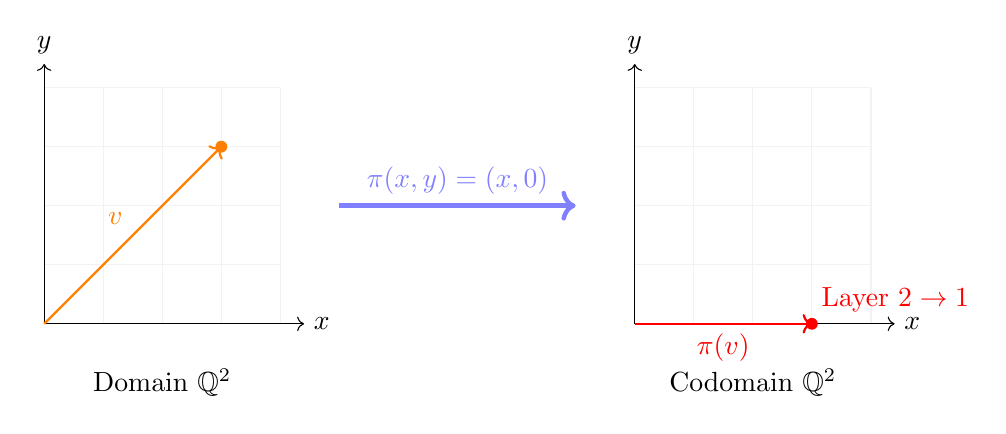
\begin{tikzpicture}[scale=1.5]
    % Domain
    \draw[step=0.5,gray!10] (0,0) grid (2,2);
    \draw[->] (0,0) -- (2.2,0) node[right] {$x$};
    \draw[->] (0,0) -- (0,2.2) node[above] {$y$};
    \node at (1, -0.5) {Domain $\Q^2$};
    
    \draw[->, thick, orange] (0,0) -- (1.5, 1.5) node[midway, above left] {$v$};
    \fill[orange] (1.5, 1.5) circle (0.05);

    % Map arrow
    \draw[->, ultra thick, blue!50] (2.5, 1) -- (4.5, 1) node[midway, above] {$\pi(x,y) = (x,0)$};

    % Codomain
    \begin{scope}[shift={(5,0)}]
        \draw[step=0.5,gray!10] (0,0) grid (2,2);
        \draw[->] (0,0) -- (2.2,0) node[right] {$x$};
        \draw[->] (0,0) -- (0,2.2) node[above] {$y$};
        \node at (1, -0.5) {Codomain $\Q^2$};

        % Projected vector
        \draw[->, thick, red] (0,0) -- (1.5, 0) node[midway, below] {$\pi(v)$};
        \fill[red] (1.5, 0) circle (0.05);
        
        \node[red, right] at (1.5, 0.2) {Layer $2 \to 1$};
    \end{scope}
\end{tikzpicture}
\caption{射影による層の降下。Layer 2のベクトルがLayer 1へ写される。}
\end{figure}

\section{基本定理の再解釈}

\subsection{線形独立性 (Exercise 5)}
Leanファイル内の定理 \texttt{linearIndependence\_iff\_minimal\_representation} は、線形独立性を「最小表現の一意性」と結びつけています。
通常、線形独立性は $\sum c_i v_i = 0 \implies c_i = 0$ で定義されますが、構造塔の文脈では、
「ベクトル $v$ の複雑さが、それを構成する基底の数と正確に一致する」
状態と捉え直すことができます。

\subsection{次元と最大層}
空間の次元（Dimension）は、構造塔における「最大の層番号」に対応します。
\[ \dim(V) = \max_{v \in V} (\minLayer(v)) \]
これは、空間内で「最も複雑なベクトル」を表現するのに必要な基底の数と言い換えられます。

\subsection{ランク・退化次数の定理 (Rank-Nullity)}
\texttt{rank\_nullity\_tower\_version} として言及されている通り、この定理は構造塔の言葉では次のように表現できる可能性があります。
\[ \text{maxLayer}(\ker f) + \text{maxLayer}(\text{im } f) = \text{maxLayer}(V) \]
これは、写像 $f$ によって「潰された次元（核）」と「残った次元（像）」の和が元の空間の複雑さに等しいことを示しています。

\section{発展：対角化と構造同型}

Leanファイルの最後では、対角化可能性（Diagonalizability）についても触れられています。
行列 $A$ が対角化可能であるとは、固有ベクトルからなる基底が存在することです。
構造塔の視点では、これは以下のように解釈されます。

\begin{theorem}[対角化と構造同型]
線形変換 $T$ が対角化可能であることは、$T$ の固有空間分解によって作られる構造塔が、標準基底による構造塔と「同型（Isomorphic）」であることと同値である。
\end{theorem}

つまり、座標系をうまくとりなおす（基底変換する）ことで、その変換の作用が各座標軸上の単純なスカラー倍（拡大縮小）として表現できる状態、それが対角化です。

\section{まとめ}
\texttt{P2.md} で示されたアプローチは、線形代数の諸概念（基底、次元、写像、対角化）を、
「ベクトルの複雑さ」と「階層構造」という統一的な視点から再構成するものです。
これにより、抽象的なベクトル空間の構造が、より具体的な「構築プロセス」として可視化されます。

\end{document}